\subsection{角域}

给定两条不同的闭射线 \(\Delta_{1}, \Delta_{2}\) ，其端点为 \(o\) ，设 \(x\) 为角 \((\widehat{\Delta_{1}, \Delta_{2}})\) 的主测度（相对于一个基 \(a\) ，一经选定便不再改变）。闭（相应地开）射线 \(\Delta\) （以 \(o\) 为端点）当中，其主测度 \(y\) （角 \((\widehat{\Delta_{1}, \Delta})\) 的）满足 \(o \leqslant y \leqslant x\) （相应地 \(o < y < x\) ）者的并集，就是代数中所定义的闭（相应地开）角域 \(S\) （以 \(\Delta_{1}\) 为始边、以 \(\Delta_{2}\) 为终边）。因为借助于一个旋转，总可以化归为 \(S\) 不包含过点 \(-1\) 的射线的情形。若 \(\alpha\) 与 \(\beta\) 此时是 \(\Delta_{1}\) 与 \(\Delta_{2}\) 分别与实正半轴所成的角，则闭角域 \(S\) 是诸闭半直线 \(\Delta\) 的并，这些半直线与实正半轴成角 \(\theta\) ，使得 \(\tan \frac{1}{2} \alpha \leqslant \tan \frac{1}{2} \theta \leqslant \tan \frac{1}{2} \beta\) 。而若 \(u, v, t\) 分别是 \(\alpha, \beta, \theta\) 的属于区间 \([- \frac{1}{2} a, + \frac{1}{2} a[\) 的测度，则这些不等式等价于 \(\tan_{a} \frac{1}{2} u \leqslant \tan_{a} \frac{1}{2} t \leqslant \tan_{a} \frac{1}{2} v\) ；又由于 \(\tan_{a} x\) 在区间 \([- \frac{1}{4} a, + \frac{1}{4} a[\) 中是递增函数，它们也等价于 \(u \leqslant t \leqslant v\) ，或等价于 \(o \leqslant t - u \leqslant v - u\) ；由于 \(x = v - u\) ，\(y = t - u\) ，于是结论对闭角域得证，而对开角域的证明是类似的。

闭角域是 \(R^{2}\) 中的闭集，而与它有同一始边和同一终边的开角域是它在 \(R^{2}\) 中的内部（第六章，§ 2，第 3 号，命题 3）。角 \((\widehat{\Delta_1, \Delta_2})\) （其主测度为 \(x\) ）称为角域 S 的角；当 \(x < \frac{1}{2} a\) 时称 S 为凸角域，当 \(x = \frac{1}{2} a\) 时称为平角域（即闭半平面），当 \(x > \frac{1}{2} a\) 时称为凹角域。凸角域当 \(x < \frac{1}{4} a\) 时为锐角域，当 \(x = \frac{1}{4} a\) 时为直角域，当 \(x > \frac{1}{4} a\) 时为钝角域。角域 S 的平分线是射线 \(\Delta\) ，它以 \(y = \frac{1}{2} x\) 为其与 \(\Delta_1\) 所成的角。

\pandocbounded{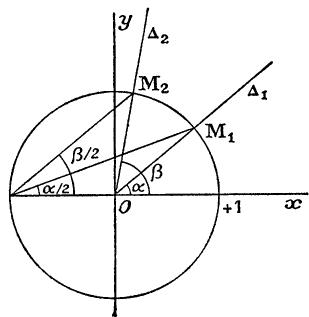
\includegraphics[keepaspectratio]{images/part001_1c4c55ab.jpg}}\\
图 10.

两条不同的闭射线 \(\Delta_{1}, \Delta_{2}\) 确定两个闭角域；它们的并是实平面 \(R^{2}\) ，而它们的交是 \(\Delta_{1} \cup \Delta_{2}\) 。

